\section{Αλγόριθμος Αποικίας Μυρμηγκίων σε βάθος}
\selectlanguage{greek}
Ο Αλγόριθμος Αποικίας Μυρμηγκιών (\lt{Ant Colony Optimization Algorithm - ACO}) είναι ένας μετευρετικός αλγόριθμος βελτιστοποίησης που έχει ως στόχο την εύρεση βέλτιστης διαδρομής σε κάποιο πρόβλημα. Μετευρετικούς (\lt{meta-heuristic}) ονομάζουμε τους αλγόρι-θμους που είναι βασισμένοι σε ευφυείς επαναληπτικές τεχνικές και αντί να ακολουθούν έναν αυστηρό κανόνα, εξάγουν γνώση με τρόπους που είναι εμπνευσμένοι από συμπεριφορές στην φύση. Συγκεκριμένα, ο \lt{ACO} είναι βασισμένος στην συμπεριφορά τον μυρμηγκιών για την αναζήτηση τροφής. 
Τα μυρμήγκια έχουν την ικανότητα να βρίσκουν πάντα την βέλτιστη διαδρομή (\lt{optimal path}) προς την πηγή τροφής όσο δύσκολο κι αν είναι αυτό. Κατά συνέπεια κι ο \lt{ACO} είναι ικανός να εντοπίζει ικανοποιητικές λύσεις σε περίπλοκα προβλήματα εκμεταλλευόμενος τις ευρετικές πληροφορίες (\lt{heuristic information}) και να εξερευνεί μεγάλους χώρους αναζήτησης σε μικρό χρονικό διάστημα αξιοποιώντας τα μονοπάτια φερομόνης (\lt{pheromone trails}) \cite{mavrovouniotis2017survey}. Όπως αναφέρθηκε και στο προηγούμενο κεφάλαιο, όταν τα μυρμήγκια κινούνται στο χώρο αφήνουν φερομόνη (\lt{pheromone}). Αυτή η ουσία αποτελεί και τρόπο επικοινωνίας μεταξύ των μυρμηγκιών, για εύρεση βέλτιστης διαδρομής προς την τροφή, αφού όσο περισσότερη φερομόνη υπάρχει σε μία διαδρομή, τόσο αυξάνεται κι η πιθανότητα ένα επόμενο μυρμήγκι να ακολουθήσει αυτή τη διαδρομή. Στον αλγόριθμο που θα υλοποιήσουμε κάθε τεχνητό μυρμήγκι αντιπροσωπεύει και μία πιθανή λύση του προβλήματος \cite{mavrovouniotis2017survey}. 


\subsection{Βασική Θεωρία}
Τα τεχνητά μυρμήγκια που χρησιμοποιούνται στον \lt{ACO} είναι εμπνευσμένα από την συμπεριφορά των πραγματικών μυρμηγκιών και αποτελούν διαδικασίες κατασκευής στοχαστικών λύσεων. Οι διαδικασίες αυτές, με χρήση πιθανολογικών τεχνικών και χρησιμοποιώντας μία δυναμική δομή μνήμης που συσχετίζεται με την ποιότητα της λύσης του προηγούμενου ληφθέντος αποτελέσματος επιλύουν υπολογιστικά προβλήματα, όπως αυτό της εύρεσης βέλτιστου μονοπατιού μέσω γράφων. Επιπλέον, προσθέτουν επαναληπτικά στοιχεία σε επιμέρους λύσεις λαμβάνοντας υπόψη ευρετικές πληροφορίες σχετικά με την επίλυση του προβλήματος και (τεχνητές) διαδρομές φερομόνης που αλλάζουν δυναμικά στο χρόνο εκτέλεσης\selectlanguage{english}\footnote{Ένα καλό εισαγωγικό βίντεο: Inspiration of Ant Colony Optimization,\\ link: \url{https://www.youtube.com/watch?v=1qpvpOHGRqA&t=784s}} \cite{dorigo2003ant, mavrovouniotis2017survey}.

\subsection{Μαθηματικό υπόβαθρο}

\begin{figure}[ht]
    \begin{minipage}[c]{.46\linewidth}
        \centering
        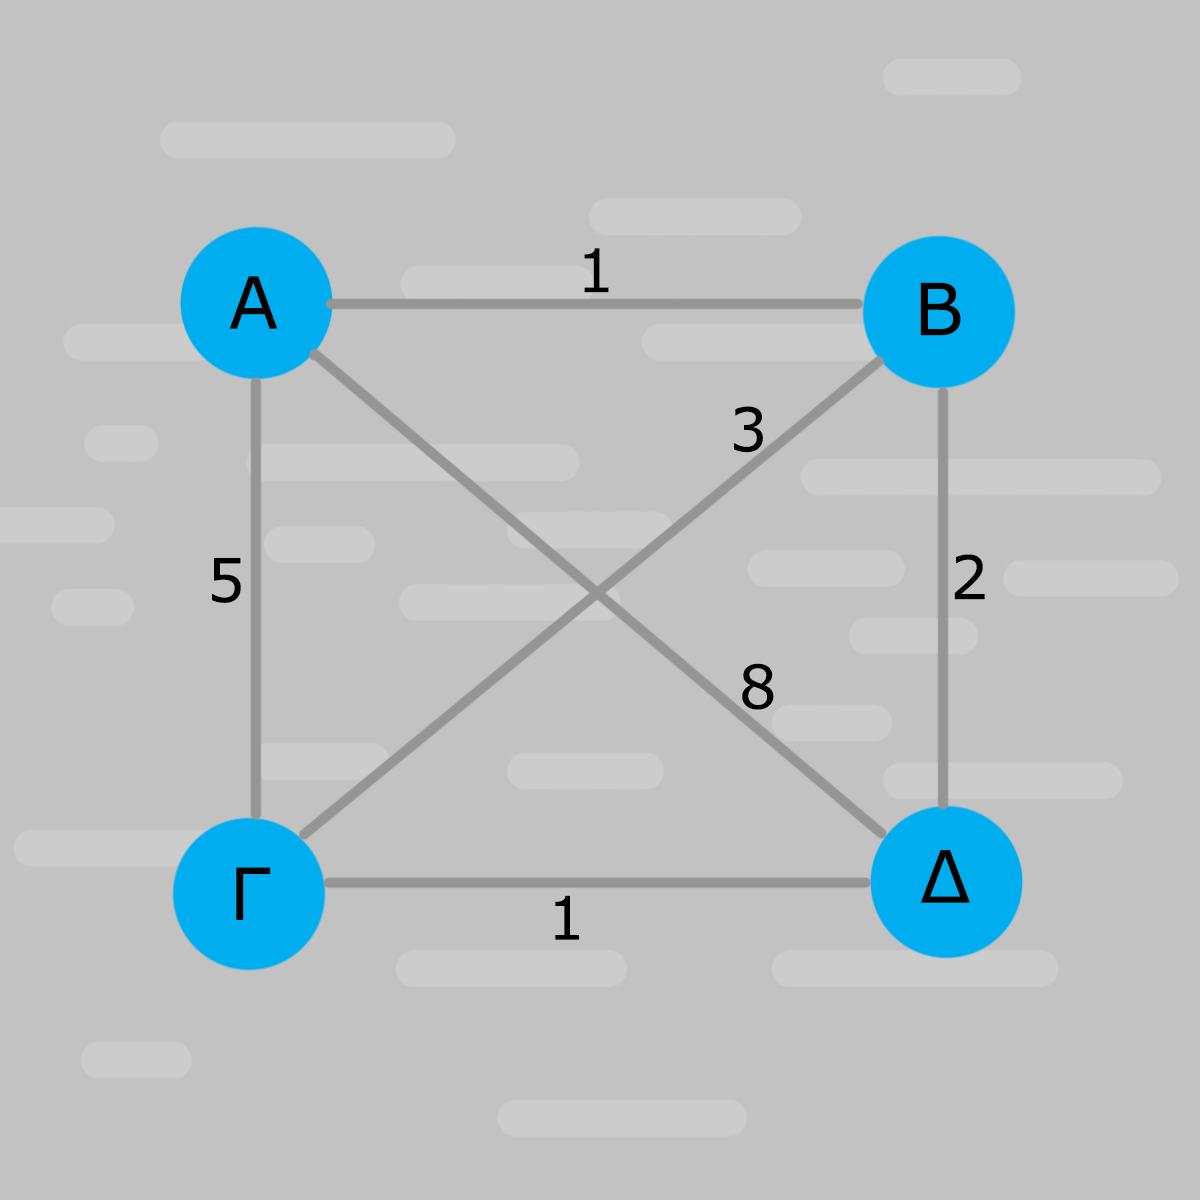
\includegraphics[scale=0.15]{2947_thesis/pictures/apostaseis.png}
        \caption{Απόσταση}
        \label{distance}
    \end{minipage}
    \begin{minipage}[c]{.46\linewidth}
        \centering
        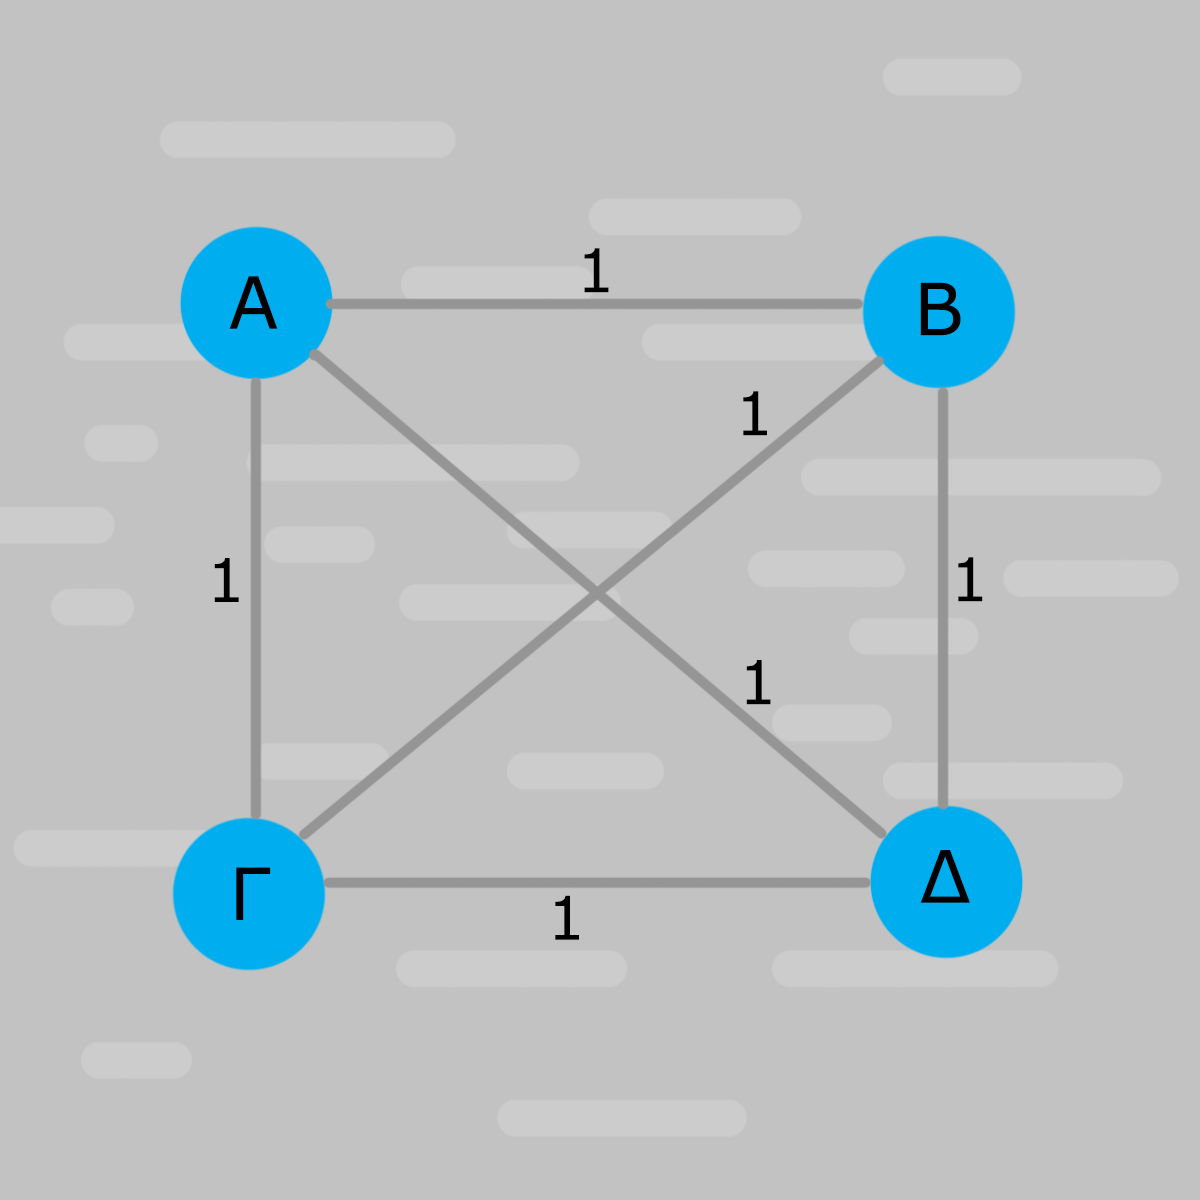
\includegraphics[scale=0.15]{2947_thesis/pictures/feromoni.png}
        \caption{Φερομόνη}
        \label{pher}
    \end{minipage}
\end{figure}
\subsubsection{Απόσταση}
Όπως αναφέρθηκε και στην δεύτερη ενότητα, ο γράφος (\lt{graph}) είναι ένα απαραίτητο κομμάτι για τη μοντελοποίηση προβλημάτων με χρήση του αλγόριθμου αποικίας μυρμηγκιών (\lt{ACO}). Η απόσταση (\lt{distance}), ή αλλιώς κόστος επιλογής μιας διαδρομής (\lt{cost}), όπως και η φερομόνη (\lt{pheromone}), θα μοντελοποιηθούν με χρήση αναπαράστασης γράφων σε πίνακα. Κάθε ακμή (\lt{edge}) του γράφου έχει ένα κόστος που συμβολίζει την απόσταση ή την γενικότερη ποιότητα της διαδρομής μεταξύ δύο κορυφών (\lt{vertices}). Έστω οι κορυφές Α, Β, Γ, Δ που ενώνονται μεταξύ τους όπως φαίνεται στο σχήμα \ref{distance} το οποίο αποτυπώνεται στον παρακάτω πίνακα γειτνίασης ως εξής:
$$
Distance = 
 \begin{array}{c|c c c c}
    & A & B & Γ & Δ \\ \hline
    A & 0 & 1 & 8 & 5 \\
    B & 1 & 0 & 2 & 3 \\
    Γ & 8 & 2 & 0 & 1 \\
    Δ & 5 & 3 & 1 & 0 
 \end{array}
 $$
 Πρόκειται για έναν μη κατευθυνόμενο γράφο (\lt{undirected graph}), δηλαδή συμμετρικό πίνακα και έχει βάρη (\lt{weight}) σε κάθε ακμή που υποδηλώνουν το κόστος επιλογής της κάθε διαδρομής, είτε αυτό εκφράζεται ως απόσταση (\lt{distance}), είτε με κάποιον άλλον τρόπο.
 
\subsubsection{Φερομόνη}
\label{3.2.2}
Τα μυρμήγκια αφήνουν φερομόνη (\lt{pheromone}) απ' όπου περνούν ανάλογα με την ποιότητα της λύσης που βρήκαν. Σε καλύτερες λύσεις συσσωρεύεται περισσότερη φερομόνη από τις υπόλοιπες. Τα μονοπάτια φερομόνης εκφράζονται ως αριθμητικές πληροφορίες μέσω ενός πίνακα, που χρησιμοποιούν τα επόμενα μυρμήγκια για την κατασκευή πιθανών λύσεων στο εκάστοτε πρόβλημα και οι οποίες πληροφορίες μεταβάλλονται κατά την εκτέλεση του αλγορίθμου με στόχο της εύρεση του βέλτιστου μονοπατιού \cite{dorigo2003ant}. Σε μονοπάτια που το μυρμήγκι επιστρέφει σε σύντομο χρονικό διάστημα συσσωρεύεται περισσότερη φερομόνη από άλλα μονοπάτια. Υπάρχουν μοντέλα που παράγουν περισσότερη φερομόνη ανάλογα με την ποιότητα αυτής της διαδρομής (για παράδειγμα την απόσταση, την ποσότητα της τροφής, και άλλα).
 
Το μαθηματικό μοντέλο αναπαράστασης της φερομόνης (\lt{pheromone model}) που εξάγει το $κ-$οστό μυρμήγκι στην ακμή που ενώνει τις κορυφές $i$ και $j$ (δηλαδή η ποσότητα της φερομόνης που παράγει, έστω $Δτ^k_{i,j}$) είναι αντιστρόφως ανάλογη με την απόσταση (ή το γενικό κόστος) της διαδρομής που διένυσε το μυρμήγκι και προκύπτει από τον τύπο, δείτε \cite{ribeiro2002ant, mpikou2013euretikoi}:
\begin{center}
    $Δτ^k_{i,j} =
    \begin{cases}
      \frac{Q}{L_k} & \text{αν $(i,j) \in τ_k$}\\
      0 & \text{αν $(i,j) \notin τ_k$}
    \end{cases}$
\end{center}
	
Όπου:
\begin{itemize}
    \item $Q$: παράμετρος που καθορίζεται από εμάς ανάλογα με το πρόβλημα, για παράδειγμα 1, 2, κλπ,
    \item $τ_k$: η διαδρομή του μυρμηγκιού $k$,
    \item $L_k$: Το συνολικό μήκος της διαδρομής $τ_k$.
\end{itemize}
Έστω ότι για το πρώτο μυρμήγκι (δηλαδή $k=1$) ο πίνακας με την φερομόνη είναι παντού 1 όπως φαίνεται στο σχήμα \ref{pher}. Με αποτέλεσμα η επιλογή διαδρομής να μην λαμβάνει υπόψην την φερομόνη. Στο παράδειγμα μας προκύπτει ο πίνακας: 
$$
Pheromone = 
 \begin{array}{c|c c c c}
    & A & B & Γ & Δ \\ \hline
    A & 0 & 1 & 1 & 1 \\
    B & 1 & 0 & 1 & 1 \\
    Γ & 1 & 1 & 0 & 1 \\
    Δ & 1 & 1 & 1 & 0 
 \end{array}
 $$
Οπότε ως εδώ έχουμε ένα χάρτη με τα πιθανά μονοπάτια στον πίνακα \lt{distance}, όπου εκφράζει το κόστος (\lt{cost}) της κάθε διαδρομής, και έναν ακόμα με την "επιθυμία" του μυρμηγκιού να επιλέγει το κάθε μονοπάτι στον πίνακα \lt{pheromone}.

Για να υπολογίσουμε την ποσότητα φερομόνης από μια κορυφή σε μία άλλη (χωρίς εξάτμιση- θα αναλυθεί παρακάτω) υπολογίζουμε το άθροισμα της φερομόνης που εξήγαγαν $m$ μυρμήγκια που πέρασαν από την κορυφή $i$ στην $j$. Δηλαδή: 
\begin{align}
    τ_{i,j}^k=\sum_{k=1}^{m}{Δτ^k_{i,j}}
\end{align}

\begin{figure}
    \centering
    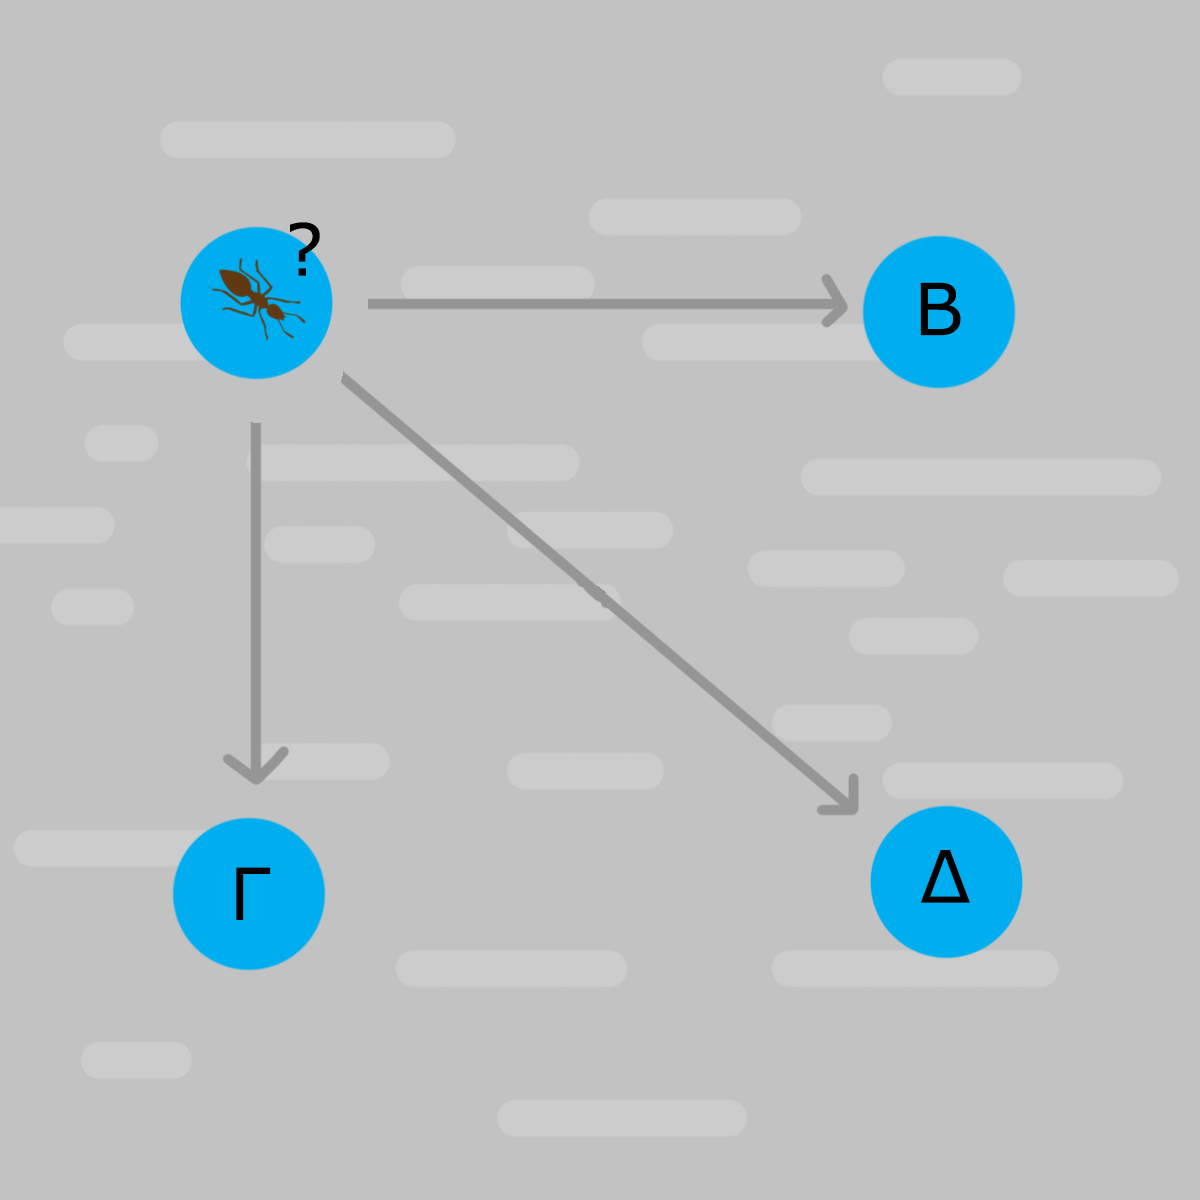
\includegraphics[scale=0.20]{2947_thesis/pictures/epilogi.png} 
    \caption{Πιθανές επιλογές}
    \label{10}
\end{figure}

\subsubsection{Επιλογή Διαδρομής}
\label{3.2.3}
Στο παράδειγμα μας ας υποθέσουμε ότι ένα μυρμήγκι ξεκινάει στην κορυφή Α. Οι πιθανές του επιλογές όπως φαίνεται και στο σχήμα \ref{10} είναι οι Β, Γ, Δ. Ποιά είναι όμως η βέλτιστη; 
Σε ένα τόσο απλό πρόβλημα, είναι εύκολο να αντιληφθούμε ενστικτωδώς ποια διαδρομή πρέπει να ακολουθήσει το μυρμήγκι, όμως αυτό δεν είναι εφικτό σε πιο περίπλοκα προβλήματα με μεγάλο πλήθος κορυφών. Έστω ότι ο αριθμός των κορυφών είναι $n$, τότε επιλέγοντας μία κορυφή ως αρχική ο αριθμός των πιθανών κορυφών γίνεται $n-1$. Αφού το μυρμήγκι επιλέξει μία από αυτές μετά θα αφαιρεθεί από τις πιθανές αφού την επισκέφθηκε και θα γίνουν $n-2$. Έτσι θα επιλέγει μονοπάτια μέχρι να μην μείνει κανένα διαθέσιμο και να επιστρέψει στο αρχικό. Άρα ο αριθμός των πιθανών επιλογών είναι $(n-1)(n-2)(n-3)\cdots3\cdot2\cdot1 = (n-1)!$. Όμως δεδομένου ότι διαδρομές όπως $A \rightarrow B \rightarrow Γ \rightarrow Δ \rightarrow A$ είναι ίδια με την $A \rightarrow Δ \rightarrow Γ \rightarrow B \rightarrow A$ πρέπει να μην επαναλαμβάνονται. Οπότε αφού πρόκειται για συμμετρικό πρόβλημα ο τύπος των πιθανών μονοπατιών γίνεται $(n-1)!/2$ αφαιρώντας τις επαναλαμβανόμενες λύσεις όπως και στο πρόβλημα του πλανόδιου πωλητή (\lt{Travelling Salesman Problem - TSP}) που θα δούμε σε επόμενο κεφάλαιο\footnote{Όπως εύστοχα περιγράφετε στο βίντεο: Ant colony optimization algorithm, \\
link: \url{https://www.youtube.com/watch?v=u7bQomllcJw}}.
Η πιθανότητα το $κ-$οστό μυρμήγκι να επιλέξει ένα μονοπάτι συμβολίζεται ως: $P^k_{i,j}$ και δίνεται από τον τύπο, δείτε \cite{chandrashekar2023hwacoa, blum2005ant}:

\begin{align} \label{eq:3}
	P^k_{i,j}=\frac{(τ_{i,j})^\alpha(η_{i,j})^\beta}{\sum_{m}(τ_{i,m})^\alpha(η_{i,m})^\beta}
\end{align}

Όπου: 
\begin{itemize}
    \item $\tau_{i,j}$: το επίπεδο φερομόνης μεταξύ των κορυφών $i$ και $j$
    \item $\eta_{i,j}$: η ποιότητα της διαδρομής
    \item $m$: οι υπόλοιπες διαδρομές που μπορούσε να επιλέξει το μυρμήγκι
    \item $\alpha, \beta$: σταθερές που επιλέγουμε ανάλογα από την επιρροή που θέλουμε να έχει το $\tau$ και το $\eta$ στην διαδικασία επιλογής (για παράδειγμα αν θέλουμε να επιλέξουμε μια διαδρομή βασισμένη αποκλειστικά και μόνο στο επίπεδο της φερομόνης τότε αφαιρούμε από την εξίσωση το $\eta_{i,j}$ θέτοντας το $\beta=0$).
\end{itemize}
Ο συμβολισμός της πιθανότητας επιλογής ενός μονοπατιού ποικίλει από βιβλιογραφία σε βιβλιογραφία. 
Το γινόμενο των $\tau_{i,j}\cdot\eta_{i,j}$ μας δίνει την "επιθυμία" (\lt{desire}) του μυρμηγκιού να επιλέξει το μονοπάτι $i \rightarrow j$.

Στο παράδειγμα μας, αφού υπολογίσουμε την "επιθυμία" του μυρμηγκιού να επιλέξει το κάθε μονοπάτι έχουμε:

\begin{enumerate}
    \item AΒ $= \tau_{A,B}\eta_{A,B}=1\cdot\frac{1}{1}=1$ 
    \item AΓ $= \tau_{A,Γ}\eta_{A,Γ}=1\cdot\frac{1}{5}=0.2$
    \item AΔ $= \tau_{A,Δ}\eta_{A,Δ}=1\cdot\frac{1}{8}=0.125$
\end{enumerate}

Όπου οι αντίστοιχες πιθανότητες γίνονται:

\begin{enumerate}
    \item $P_{A,B}=\frac{1}{1+0.125+0.2}=\frac{1}{1.325}=0.75...$
    \item $P_{A,Γ}=\frac{0.2}{1.325}=0.15...$
    \item $P_{A,Δ}=\frac{0.125}{1.325}=0.09...$
\end{enumerate}

Βλέπουμε ότι πιο πιθανό είναι το μυρμήγκι να επιλέξει την διαδρομή Α $\rightarrow$ Β όμως υπάρχει μικρή πιθανότητα να επιλέξει και τις υπόλοιπες. Για την επιλογή της περιοχής χρησιμοποιώντας την πληροφορία που αντλούμε από αυτές τις πιθανότητες, αντί να χρησιμοποιήσουμε μόνο την εντολή \lt{random} που μας παρέχει η \lt{python} για τυχαία επιλογή, θα χρησιμοποιήσουμε την τεχνική \lt{roulette wheel select} \cite{lipowski2012roulette}. Αρχικά υπολογίζουμε το άθροισμα των πιθανοτήτων επιλογής κάθε διαδρομής. Αφού μιλάμε για πιθανότητες το άθροισμα αυτό θα είναι πάντα 1. Έπειτα, επιλέγουμε τυχαία έναν αριθμό εντός αυτού του συνόλου, δηλαδή $[0,1]$, και βρίσκουμε την διαδρομή στην οποία αντιστοιχεί αυτός ο αριθμός.
Στην υλοποίησή μας η εντολή: \verb|roulette_wheel_select()| θα επιλέγει μία κορυφή τυχαία με βάση τις πιθανότητες επιλογής τους. Ο κώδικας που υλοποιεί αυτήν την διαδικασία είναι ο παρακάτω: 
\lstinputlisting[language=python]{code/roulette_wheel.py}
Όπου:
\begin{itemize}
    \item \verb|random_prob|: ένας τυχαίος αριθμός με τον οποίο θα γίνει επιλογή κορυφής που θα πάει το μυρμήγκι.
    \item \verb|current|: ο δείκτης των περιοχών.
\end{itemize}

Στο παράδειγμά μας από 0 έως 0,76 αντιστοιχεί στην διαδρομή Α $\rightarrow$ Β, από το 0,77 έως το 0,91 αντιστοιχεί στην διαδρομή Α $\rightarrow$ Γ και απο το 0,92 έως το 1 στην διαδρομή Α $\rightarrow$ Δ. Οπότε αν για παράδειγμα επιλεγόταν ο αριθμός 0,41 θα επέλεγε το μονοπάτι (ακμή) Α $\rightarrow$ Β όπως φαίνεται στο σχήμα \ref{roulette}.

\begin{figure}[b]
    \centering
    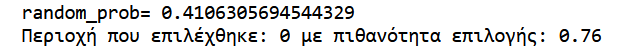
\includegraphics[scale=0.9]{2947_thesis/pictures/roulette_wheel_example.png} 
    \caption{Παράδειγμα roulette wheel}
    \label{roulette}
\end{figure}

\subsubsection{Εξάτμιση Φερομόνης}

Η διαδικασία της εξάτμισης φερομόνης (\lt{evaporation}) είναι ένα σημαντικό κομμάτι για την απόδοση του αλγόριθμου και την εύρεση της βέλτιστης λύσης. Όταν όλα τα μυρμήγκια έχουν ολοκληρώσει την διαδρομή τους, ο πίνακας με τις φερομόνες (\lt{pheromone}) πρέπει να ανανεωθεί. Αυτό γίνεται μέσω εξάτμισης της φερομόνης με ένα σταθερό ρυθμό $ρ \in [0,1]$ (\lt{evaporation rate}) που καθορίζουμε εμείς. Ένας υψηλός ρυθμός εξάτμισης υποδηλώνει γρήγορη εξάτμιση ενώ ένα χαμηλός αργή. Το πόσο γρήγορα εξατμίζεται η φερομόνη επηρεάζει τη συμπεριφορά των μυρμηγκιών σε μεγάλο βαθμό \cite{dawson2013improving}. Εμείς θα έχουμε $ρ=0.5$ (Όπως προτείνεται από τους \lt{Dorigo and Stutzle}) \cite{dorigo2003ant}. Ο τύπος της εξάτμισης την χρονική στιγμή $t$ είναι \cite{blum2005ant, mpikou2013euretikoi}:

\begin{align}
	τ_{i,j}(t)\leftarrow(1-ρ)τ_{i,j}(t-1).
\end{align}

Αυτό επιτρέπει σε λύσεις που δεν είναι ιδανικές να μην λαμβάνονται υπόψιν. Όπως αναφέρθηκε και στο κεφάλαιο \nameref{3.2.2}, ο τύπος για τον υπολογισμό της φερομόνης από μία κορυφή σε μία άλλη είναι: 
\begin{align}
    τ_{i,j}^k=\sum_{k=1}^{m}{Δτ^k_{i,j}}
\end{align}
Με εξάτμιση αυτός γίνεται: 
\begin{align}
    τ_{i,j}^k\leftarrow(1-ρ)τ_{i,j}+\sum_{k=1}^{m}{Δτ^k_{i,j}}
\end{align}
Όπου: 
\begin{itemize}
    \item $τ_{i,j}$ η ποσότητα της φερομόνης στην προηγούμενη επανάληψη,
    \item $1-ρ$ ο ρυθμός εξάτμισης,
    \item $\sum_{k=1}^{m}{Δτ^k_{i,j}}$ το άθροισμα φερομόνης που άφησαν όλα τα $m$ μυρμήγκια που πέρασαν από την ακμή $i\rightarrow j$
\end{itemize}
Η εξάτμιση της φερομόνης ευνοεί την εξερεύνηση νέων περιοχών στον χώρο αναζήτησης. Υπάρχει μεγάλο πλήθος διαφορετικών \lt{ACO} με μόνη διαφορά τον τρόπο που γίνεται η ενημέ- ρωση της φερομόνης \cite{mpikou2013euretikoi}.

\subsubsection{Πλάνο Αλγορίθμου}
Το πλάνο του αλγόριθμου παρουσιάζεται στην εικόνα \ref{plan}.
\begin{figure}
    \centering
    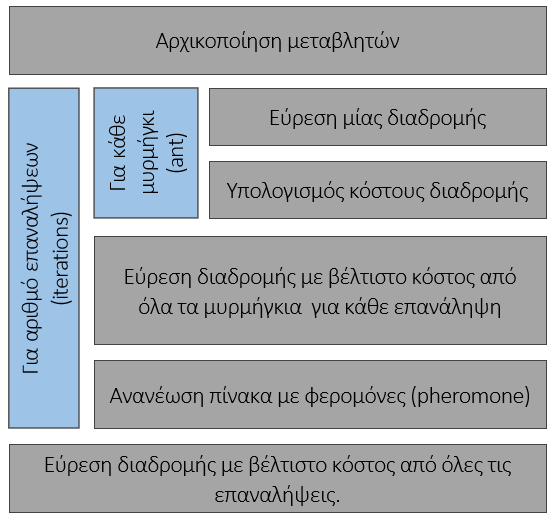
\includegraphics[scale=0.80]{2947_thesis/pictures/plan.png} 
    \caption{Πλάνο Αλγόριθμου.}
    \label{plan}
\end{figure}

\subsection{Υλοποίησή μου Αλγορίθμου σε python}
\selectlanguage{greek}
Αφού κάνουμε \lt{import} τις απαραίτητες βιβλιοθήκες, γίνεται αρχικοποίηση των μεταβλητών που θα χρειαστούμε. Αυτές είναι: το πλήθος των διαθέσιμων περιοχών που μπορούν να επισκεφτούν τα μυρμήγκια (\lt{areas}), το πλήθος των μυρμηγκιών (\lt{ants}), ο αριθμός των επαναλήψεων που θα εκτελέσει ο αλγόριθμος (\lt{iterations}) και οι σταθερές $\alpha$ και $\beta$ (\lt{alpha, beta}). Ο κώδικας που θα παρουσιαστεί μπορεί να βρεθεί ολόκληρος στο link: \url{https://github.com/vaggbik/ant_colony_algorithm}.
\lstinputlisting[language=python]{code/step1.py}

Έπειτα δημιουργούμε τον πίνακα με τον οποίο θα μοντελοποιήσουμε το κόστος επιλογής κάθε μονοπατιού (\lt{distance}). Αυτό το κάνουμε τυχαία επιλέγοντας έναν αριθμό από το 0 έως το 50 για κάθε ακμή του γράφου.
\lstinputlisting[language=python]{code/step2_1.py}

Πρόκειται για έναν μη κατευθυνόμενο γράφο (\lt{undirected graph}) οπότε πρέπει να τον μετατρέψουμε σε συμμετρικό, αυτό το κάνουμε προσθέτοντας τον πίνακα \lt{distance} με τον ανάστροφο (\lt{transposed}) πίνακα $distance^{Transposed}$ και διαιρούμε με το 2, επίσης αφαιρούμε τους βρόχους (ακμές που ξεκινάν και τελειώνουν στην ίδια κορυφή) θέτοντας 0 στα κελιά $(i,i)$, όπου $i\in[0,\rm{areas})$ \cite{perez2020introduction}.
\lstinputlisting[language=python]{code/step2_2.py}

Γίνεται αρχικοποίηση του πίνακα με τις φερομόνες (\lt{pheromone}) να έχει παντού 1. Στην πρώτη επανάληψη του αλγορίθμου η επιλογή διαδρομής από ένα μυρμήγκι θα εξαρτάται μόνο από τον πίνακα κόστους της διαδρομής (\lt{distance}). 
\lstinputlisting[language=python]{code/step3.py}

Έπειτα για όσες φορές θέλουμε να εκτελέσουμε τον αλγόριθμο (\lt{iterations}),
τοποθετού- με το κάθε μυρμήγκι σε μια τυχαία περιοχή ως αρχική του, αυτό το κάνουμε δημιουργώντας μια λίστα (\lt{ant\_areas}) μεγέθους όσα και τα μυρμήγκια και επιλέγοντας μία τυχαία περιοχή για το καθένα με χρήση της \lt{randint} \cite{w3school}.
\lstinputlisting[language=python]{code/step4_1.py}
Η πάνω διαδικασία μπορεί επίσης να γραφεί ως εξής: 
\lstinputlisting[language=python]{code/step4_2.py}

Στην συνέχεια κάθε μυρμήγκι επιλέγει την επόμενη περιοχή που θα επισκεφτεί για όσες περιοχές υπάρχουν (\lt{areas}) με χρήση της φερομόνης (\lt{pheromone}) και του κόστους επιλογής κάθε διαδρομής (\lt{distance}). Αυτό θα το πετύχουμε μοντελοποιώντας την συνάρτηση (\ref{eq:3}). Η τυχαία επιλογή αριθμού όπως αναφέρθηκε και στο κεφάλαιο \nameref{3.2.3} θα γίνεται με την συνάρτηση \lt{roulette\_wheel\_select()} που δημιουργήσαμε \cite{lipowski2012roulette}.
Αρχικά υπολογίζουμε τις διαθέσιμες περιοχές που μπορεί να επισκεφθεί το κάθε μυρμήγκι (\lt{available\_areas}). Έπειτα υπολογίζουμε την "επιθυμία" του κάθε μυρμηγκιού να ακολουθήσει κάθε μονοπάτι από τα διαθέσιμα και στη συνέχεια την πιθανότητα επιλογής του κάθε μονοπατιού. Αυτή την πιθανότητα την εισάγουμε ως μεταβλητή στην συνάρτηση \lt{roulette\_wheel\_select()} που δημιουργήσαμε και έχουμε ως αποτέλεσμα τον δείκτη που βρίσκεται επιλαχούσα περιοχή που θα ακολουθήσει το μυρμήγκι στον πίνακα με τις διαθέσιμες περιοχές. Αυτό το ονομάζουμε \lt{next\_area}. Τέλος προσθέτουμε τον πίνακα με τη διαδρομή κάθε μυρμηγκιού στο \lt{ant} και υπολογίζουμε το μήκος αυτών στο \lt{ant\_distances}\footnote{Xρήσιμες ιστοσελίδες-πηγές με \lt{python}: \\
link 1: \url{https://www.w3schools.com/python/}\\
link 2: \url{https://blog.teamtreehouse.com/python-single-line-loops} \\
link 3: \url{https://blog.finxter.com/python-one-line-for-loop-with-if/}\\
link 4: \url{https://stackify.com/python-tips-10-tricks-for-optimizing-your-code/}
}.
\lstinputlisting[language=python]{code/step5.py}

Έπειτα, αφού έχουμε βέλτιστη λύση από την εκτέλεση του αλγορίθμου, ανανεώνουμε τον πίνακα με τις φερομόνες έτσι ώστε καλύτερες λύσεις να είναι πιο πιθανό να επιλεγούν.
\lstinputlisting[language=python]{code/step6.py}
Όπου το $ρ=0.5$, ο ρυθμός εξάτμισης και \lt{pheromone\_sum} το $\sum_{k=1}^{m}{Δτ^k_{i,j}}$. 


Αυτή την διαδικασία την επαναλαμβάνουμε όσες φορές θέλουμε να εκτελεστεί ο αλγόρι- θμος (\lt{iterations}). Όσο μεγαλύτερο το \lt{iterations}, τόσο καλύτερη θα είναι η λύση, αφού κάθε επανάληψη αυξάνει την πιθανότητα να βρεθεί μια ακόμα καλύτερη λύση από την προηγούμενη και έχει ως αποτέλεσμα να πλησιάζουμε όλο και περισσότερο στην βέλτιστη.

Παρακάτω δίνετε ο αλγόριθμος ολοκληρωμένος:
\lstinputlisting[language=python]{code/ant_colony_algorithm.py}

\begin{table}
\begin{center}
\begin{tabular}{|c|c|}
    \hline
    {\bf Μεταβλητή} & {\bf Ιδιότητα}\\ \hline
    \lt{ants} & πλήθος μυρμηγκιών\\ \hline
    \lt{areas} & πλήθος περιοχών\\ \hline
    \lt{iterations} & πλήθος επαναλήψεων\\ \hline
    \lt{alpha} & σταθερά "α"\\ \hline
    \lt{beta} & σταθερά "β" \\ \hline
    \lt{distance} & πίνακας μεγέθους $areas \times areas$ με\\
    &  κόστος επιλογής κάθε μονοπατιού\\ \hline
    \lt{pheromone} & πίνακας μεγέθους $areas \times areas$ με\\ 
    & ποσότητα φερομόνης σε κάθε μονοπάτι\\ \hline
    \lt{ant\_areas} & λίστα μεγέθους όσα και τα\\ 
    & μυρμήγκια με αρχικές περιοχές\\
    & για το καθένα\\ \hline
    \lt{available\_areas} & διαθέσιμες περιοχές που μπορεί\\ 
    & να επισκεφτεί το κάθε μυρμήγκι\\ \hline
    \lt{probabilities} & η "επιθυμία" επιλογής κάθε\\
    & μονοπατιού από κάθε μυρμήγκι\\ \hline
    \lt{total\_pheromone} & το άθροισμα όλων των επιθυμιών\\ 
    & κάθε επανάληψης\\ \hline
    \lt{next\_area} & επιλεχούσα περιοχή με\\ 
    & χρήση roulette\_wheel\_select\\ \hline
    \lt{pheromone\_sum} & άθροισμα φερομόνης σε κάθε μονοπάτι\\ \hline
    \lt{ant\_distances} & άθροισμα κόστους διαδρομών\\ 
    & που επέλεξε το κάθε μυρμήγκι\\ \hline
    \lt{best\_route} & λίστα με καλύτερες διαδρομές\\
    & της κάθε επανάληψης\\ \hline
    \lt{best\_one\_route} & μονοπάτι καλύτερης διαδρομής\\
    & από όλες τις επαναλήψεις\\ \hline
    \lt{best\_one\_distance} & κόστος καλύτερης διαδρομής\\
    & από κάθε επανάληψη\\ \hline

\end{tabular}
\end{center}
\caption{Πίνακας με μεταβλητές αλγόριθμου}
\end{table}





\subsection{Εκτέλεση του Αλγορίθμου}
Στο παράδειγμα που εκτελέσαμε έχουμε δώσει ως δεδομένα: 5 μυρμήγκια (\lt{ants}), που εκτελούν αναζήτηση μεταξύ 5 περιοχών (\lt{areas}), 10 φορές (\lt{iterations}) με \lt{alpha} και \lt{beta} ίσα με 1, η εκτέλεση του αλγορίθμου με τα παραπάνω δεδομένα δίνουν αποτέλεσμα παρόμοιο με αυτό που φαίνεται στο σχήμα \ref{12}.

\begin{figure}
    \centering
    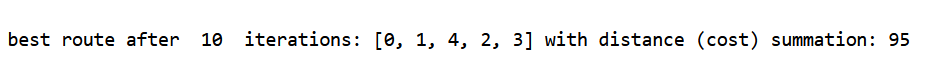
\includegraphics[scale=0.65]{2947_thesis/pictures/ex1.png} 
    \caption{Παράδειγμα με: \lt{ants}=5, \lt{areas}=5, \lt{iterations}=10, \lt{alpha=beta}=1.}
    \label{12}
\end{figure}

Ανάλογα από τις απαιτήσεις του εκάστοτε προβλήματος, οι μεταβλητές μπορούν να αλλάξουν, τί γίνεται όταν αλλάξουμε τα \lt{alpha} και \lt{beta}, τί συμβαίνει με μικρό αριθμό επαναλήψεων, πώς λειτουργεί το πρόγραμμα με εξάτμιση και πώς χωρίς εξάτμιση, πώς σχετίζεται η ποιότητα της λύσης με τον αριθμό των μυρμηγκιών; Ερωτήσεις σαν κι αυτές θα απαντηθούν παρακάτω με παραδείγματα εκτέλεσης του αλγορίθμου και με τα αντίστοιχα αποτελέσματα. 
Για εύκολη κατανόηση του προβλήματος και για τον σκοπό της επίτευξης των συγκρίσεων θα γίνει χρήση ίδιου πίνακα \lt{distance} σε όλα τα παρακάτω παραδείγματα, ο οποίος δίνεται στο σχήμα \ref{13} με βέλτιστα αποτελέσματα που φαίνονται στο σχήμα \ref{14}.
\begin{figure}
    \centering
    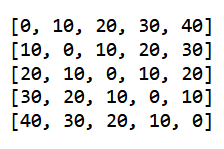
\includegraphics[scale=1]{2947_thesis/pictures/distance.png} 
    \caption{Πίνακας \lt{distance} που θα χρησιμοποιηθεί για τα παραδείγματα.}
    \label{13}
\end{figure}
\begin{figure}
    \centering
    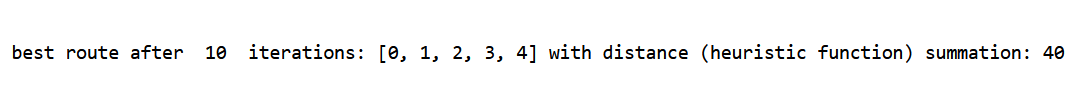
\includegraphics[scale=0.65]{2947_thesis/pictures/ex2.png} 
    \caption{Βελτιστα αποτελέσματα για είσοδο \lt{distance} της εικόνας \ref{13}.}
    \label{14}
\end{figure}

\selectlanguage{english}
\subsubsection{Τροποποίηση των alpha, beta}
\selectlanguage{greek}
Σε περίπτωση που το \lt{alpha} πάρει την τιμή 0, η επιρροή που έχει ο πίνακας με τις φερομόνες (\lt{pheromone}) μηδενίζεται, αφαιρώντας έτσι το δυνατότητα του αλγόριθμου να "μάθει" από προηγούμενες εκτελέσεις, με αποτέλεσμα ο αλγόριθμος να βασίζεται μόνο στο πίνακα με το κόστος επιλογής κάθε διαδρομής (\lt{distance}) και κατά συνέπεια στο ποιο είναι το καλύτερο μονοπάτι εκείνη την χρονική στιγμή χωρίς να δίνεται βάση σε προηγούμενες λύσεις. Το πρόγραμμα μας εξάγει πάλι βέλτιστα αποτελέσματα \ref{14}, αλλά παρατηρώντας τα, είναι εύκολα αντιληπτό ότι η λύση βρέθηκε λόγο της απλότητας του προβλήματος. 

Αντίστοιχα, αν το \lt{beta} πάρει την τιμή 0, μηδενίζεται η επιρροή του πίνακα το κόστος επιλογής κάθε διαδρομής (\lt{distance}) και το αποτέλεσμα θα βασίζεται καθαρά στον πίνακα με τις φερομόνες (\lt{pheromone}), πάλι δίνονται βέλτιστα αποτελέσματα, αυτό συμβαίνει γιατί έχουμε θέσει τον πίνακα με τις φερομόνες να είναι παντού 1, οπότε η πιθανότητα σε 10 επαναλήψεις να βρει την βέλτιστη διαδρομή είναι μεγάλη, αν γίνει αλλαγή του πίνακα με τις φερομόνες αυξάνοντας την επιρροή μιας μη βέλτιστης διαδρομής τότε παρατηρούμε ότι ενώ με \lt{alpha=beta}$=1$ καταφέρνει να ανακάμψει γρήγορα και δίνεται πάλι η βέλτιστη διαδρομή ως αποτέλεσμα όπως φαίνεται στο σχήμα \ref{14}, στην περίπτωση που το \lt{beta}$=0$ αυτό δεν συμβαίνει τόσο εύκολα, σχήμα \ref{16}.

\begin{figure}
    \centering
    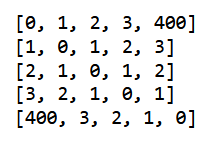
\includegraphics[scale=1]{2947_thesis/pictures/pheromone.png} 
    \caption{Πίνακας \lt{pheromone} με διαφορετικές επιρροές.}
    \label{15}
\end{figure}
\begin{figure}
    \centering
    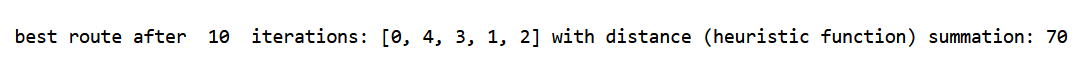
\includegraphics[scale=0.65]{2947_thesis/pictures/ex3.png} 
    \caption{Αποτελέσματα για \lt{pheromone} \ref{15} και \lt{beta}=0.}
    \label{16}
\end{figure}
Παρατηρούμε ότι τα \lt{alpha} και \lt{beta} αποτελούν σημαντικούς παράμετρους για την εύρεση λύσης καθώς επηρεάζουν το πως ο αλγόριθμος βρίσκει την βέλτιστη διαδρομή, αν είναι ιδανικά  για το εκάστοτε προβλήματα τότε η λύση θα βρεθεί γρηγορότερα. Κατά συνέπεια αν $alpha>beta$ τα μυρμήγκια εστιάζουν στις προηγούμενες λύσεις, δίνοντας έμφαση στην "μνήμη" του προγράμματος, ενώ αν $beta>alpha$ έμφαση δίνετε στην αξία της λύσης την συγκεκριμένη χρονική στιγμή. Κατά συνέπεια η ισορροπία μεταξύ αυτών των δύο παραμέτρων και η σωστή ρύθμιση τους είναι κομβικής σημασίας για την επίτευξη καλών αποτελεσμάτων. 



\subsubsection{Εξάτμιση/Ρυθμός εξάτμισης}
Άλλος ένα σημαντικός παράγοντας για την ορθή εκτέλεση του αλγόριθμου της αποικίας των μυρμηγκιών είναι ο ρυθμός εξάτμισης (\lt{evaporation rate} - $ρ$). Ο ρυθμός αυτός βοηθάει στην εξάλειψη των ιχνών φερομόνης σε μη ιδανικά μονοπάτια (αφού ενθαρρύνει την διέλευση από ανεξερεύνητες περιοχές), που πιθανών οδηγήσουν σε λάθος αποτελέσματα αφού θα αποπροσανατολίσουν τα μυρμήγκια, χωρίς όμως να έχουμε απώλεια πληροφορίας \cite{mavrovouniotis2014ant, mpikou2013euretikoi}. Ένας υψηλός ρυθμός εξάτμισης ($ρ$) υποδηλώνει ότι η φερομόνη εξατμίζεται ταχύτερα ($1-ρ$) με αποτέλεσμα να παίζει σημαντικότερο ρόλο το κόστος επιλογής κάθε διαδρομής και οι πληροφορίες που σχετίζονται με την φερομόνη από προηγούμενες επαναλήψεις να χάνονται πιο γρήγορα. Δηλαδή, δίνεται περισσότερη βάση στην εξερεύνηση του διαθέσιμου χώρου. Αντίθετα ένας πολύ χαμηλός ρυθμός εξάτμισης ($ρ$) υποδηλώνει ότι η φερομόνη θα παραμένει στις ακμές περισσότερο χρόνο με αποτέλεσμα τα μυρμήγκια να ακολουθούν τα ίδια μονοπάτια που εξερευνήθηκαν νωρίτερα.
Συνοψίζοντας, υψηλός ρυθμός εξάτμισης δίνει έμφαση στην εξερεύνηση του χώρου ενώ χαμηλός ρυθμός δίνει έμφαση στην "μνήμη" του προγράμματος. Σε περίπτωση που μηδενίσουμε την εξάτμιση παρατηρούμε ότι η σύγκλιση σε βέλτιστη λύση συνήθως καθυστερεί, αυτό συμβαίνει γιατί τα μυρμήγκια τείνουν να επιλέγουν τα ίδια μονοπάτια ακόμα κι αν δεν είναι βέλτιστα. Στο παράδειγμα μας οδηγεί πάλι στην βέλτιστη λύση \ref{14} αλλά χρειάζεται (συνήθως) περισσότερο αριθμό επαναλήψεων \cite{mpikou2013euretikoi}. Διάφορες παραλλαγές του αλγόριθμου της αποικίας των μυρμηγκιών έχουν αναπτυχθεί με μόνη διαφορά τον τρόπο με τον οποίο ενημερώνεται η φερομόνη, ένα παραδείγματα αυτού είναι ο max-min αλγόριθμος (\lt{max-min ant system}) που παρουσιάστηκε από τους \lt{Stützle} και \lt{Holger} το 2000 και είχε ως βασικό χαρακτηριστικό ότι μόνο το μυρμήγκι με την καλύτερη λύση από κάθε επανάληψη (\lt{best\_route}) επιτρεπόταν να ενημερώσει τον πίνακα με τις φερομόνες \cite{stutzle2000max}.


\subsubsection{Επαναλήψεις}
Ακόμα ένας σημαντικός παράγοντας για την εύρεση βέλτιστης λύσης είναι ο αριθμός επαναλήψεων (\lt{iterations}) που θα εκτελεστεί ο αλγόριθμος και τα μυρμήγκια θα ψάξουν για λύση. Θεωρώντας τον πίνακα με την φερομόνη μη ιδανικό, όπως φαίνεται στο σχήμα\selectlanguage{english} \ref{pher2}, δοκιμάζουμε τα εξής σενάρια:
\begin{itemize}
    \item iterations=1:
    Σε αυτή την περίπτωση, τα μυρμήγκια επηρεασμένα από την φερομόνη ακολουθούν μη βέλτιστη διαδρομή και δεν τους δίνεται χρόνος για εξάτμιση, με αποτέ- λεσμα να οδηγούμαστε πάντα σε λάθος λύση, παράδειγμα στο σχήμα \ref{iter1}.
    \item iterations=10:
    Αν αυξήσουμε τον αριθμό επαναλήψεων, παρατηρούμε ότι δίνεται χρό- νος στα μυρμήγκια να ανακάμψουν από την λάθος διαδρομή και να βελτιωθεί η ποιότητα της λύσης (πολλές φορές και στην βέλτιστη για το παράδειγμα μας), αυτό συμβαίνει αφού δίνεται ο απαραίτητος χρόνος για αντικατάσταση του πίνακα με τις φερομόνες και εξάτμιση της λανθασμένης διαδρομής, παράδειγμα στο σχήμα \ref{iter10}.
    \item iterations=100:
    \selectlanguage{greek}
    Αν αυξήσουμε ακόμα περισσότερο τον αριθμό των επαναλήψεων, παρατηρούμε ότι τα μυρμήγκια όσες φορές και να εκτελέσουμε τον αλγόριθμο πάντα καταφέρνουν να βρουν την βέλτιστη λύση στο συγκεκριμένο παράδειγμα, παράδειγμα στο σχήμα \ref{iter100}.
    \selectlanguage{english}
\end{itemize}
\begin{figure}
    \centering
    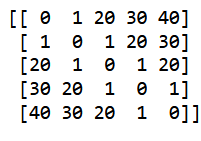
\includegraphics[scale=1]{2947_thesis/pictures/pheromone2.png} 
    \caption{Πίνακας pheromone με διαφορετικές επιρροές.}
    \label{pher2}
\end{figure}
\begin{figure}
    \centering
    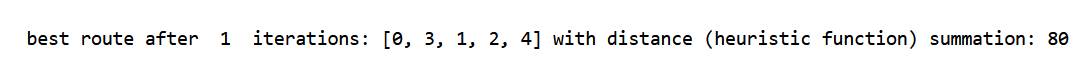
\includegraphics[scale=0.60]{2947_thesis/pictures/ex4.png} 
    \caption{Αποτελέσματα για \lt{iterations=1}.}
    \label{iter1}
\end{figure}
\begin{figure}
    \centering
    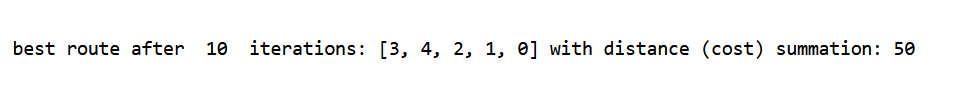
\includegraphics[scale=0.60]{2947_thesis/pictures/ex5.png} 
    \caption{Αποτελέσματα για \lt{iterations=10}.}
    \label{iter10}
\end{figure}
\begin{figure}
    \centering
    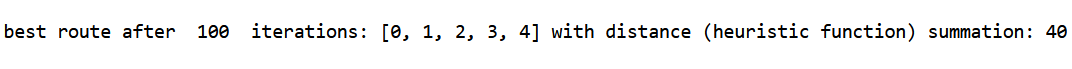
\includegraphics[scale=0.60]{2947_thesis/pictures/ex6.png} 
    \caption{Αποτελέσματα για \lt{iterations=100}.}
    \label{iter100}
\end{figure}

Τρέχοντας τον αλγόριθμο με τυχαίες μεταβλητές για 10 επαναλήψεις (iterations) και 100 αντίστοιχα για 20 περιοχές (areas) έχουμε αποτελέσματα όπως φαίνονται στις εικόνες \ref{i100} και \ref{i10} τα οποία απεικονίζουν το κόστος της καλύτερης διαδρομής μετά από κάθε επανάληψη (best\_one\_distance). Παρατηρούμε ότι όσο περισσότερες επαναλήψεις πραγματοποιηθούν τόσο πιο meμεγαλύτερη η πιθανότητα να βρεθεί καλύτερη λύση. Για παράδειγμα, στο σχήμα \ref{i100} η βέλτιστη λύση βρίσκεται μετά την επανάληψη 70.

\begin{figure}
    \centering
    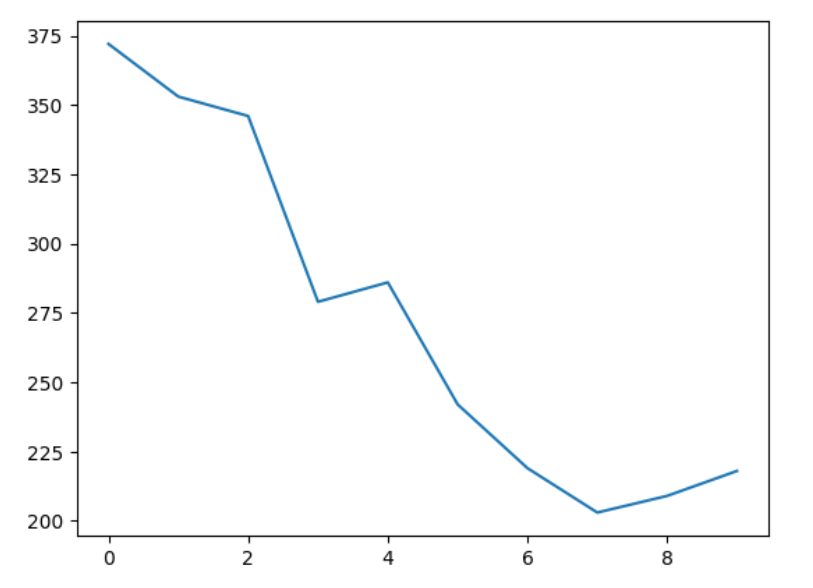
\includegraphics[scale=0.50]{2947_thesis/pictures/i10.png}
    \caption{διάγραμμα καλύτερων διαδρομών για 10 επαναλήψεις.}
    \label{i10}
\end{figure}
\begin{figure}
    \centering
    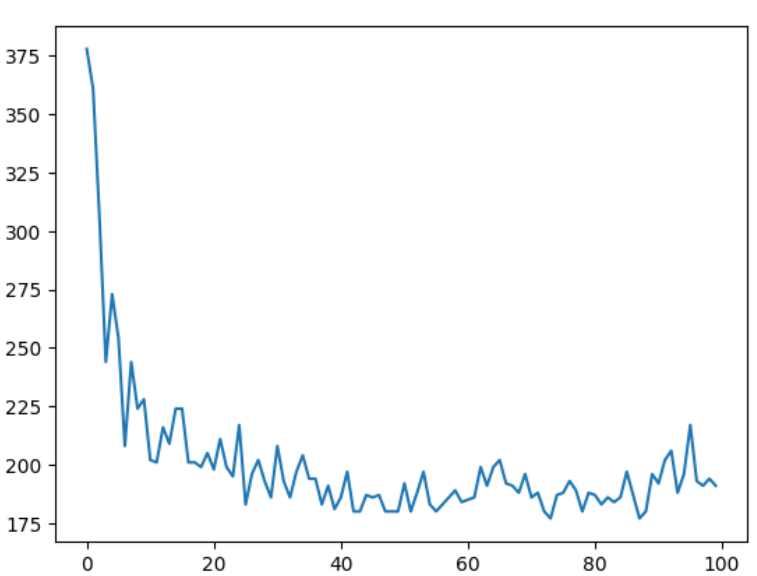
\includegraphics[scale=0.50]{2947_thesis/pictures/i100.png}
    \caption{διάγραμμα καλύτερων διαδρομών για 100 επαναλήψεις.}
    \label{i100}
\end{figure}

\subsubsection{Αριθμός μυρμηγκιών}
Ένας ακόμα σημαντικός παράγοντας στον αλγόριθμο μας είναι το πλήθος των μυρμηγ-κιών. Αυτός μπορεί να επηρεάζει αρκετά την απόδοσή του. Μεγάλο πλήθος μυρμηγκιών υ- ποδηλώνει μεγαλύτερο εύρος εξερεύνησης σε λιγότερες επαναλήψεις καθώς και γρηγορότερη σύγκλιση σε μια αποδοτική λύση, βέβαια αυξάνετε το κόστος σε υπολογιστική ισχύ κάνο- ντας τον πρόγραμμα πιο αργό στην εκτέλεση του. Αντίστοιχα, μικρό πλήθος μυρμηγκιών μπορεί να οδηγήσει σε πιο αργή σύγκλιση της λύσης στην βέλτιστη, αφού η διαδικασία ε- ξερεύνησης θα είναι πιο χρονοβόρα. Στο παράδειγμά μας, μικρός αριθμός μυρμηγκιών αρκεί για εξερεύνηση των 5 περιοχών, όσο πιο περίπλοκο γίνεται το πρόβλημα, με περισσότερες περιοχές για εξερεύνηση τόσο περισσότερα θα πρέπει να είναι και τα μυρμήγκια. Γενικά, η ιδανική τιμή του $m$ εξαρτάται από τον αλγόριθμου \lt{ACO} που έχουμε επιλέξει καθώς και από την κατηγορία προβλημάτων που στοχεύουμε να λύσουμε. Η εύρεση του βέλτιστου συνήθως γίνεται πειραματικά \cite{dorigo2003ant}.


\subsection{Εφαρμογές Αλγορίθμου}
Ο αλγόριθμος της αποικίας των μυρμηγκιών, όπως ήδη αναφέρθηκε, δίνει λύση σε πληθώρα προβλημάτων του πραγματικού μας κόσμου, όπως είναι η εύρεση βέλτιστης διαδρομή σε προ- βλήματα δρομολόγησης, η βελτιστοποίηση των δικτύων επικοινωνίας, η δρομολόγηση δι- κτύου δεδομένων, η εύρεση ακμών σε εικόνες και πολλά άλλα \cite{manwlopoulos2014thewria}. 

\subsubsection{Πρόβλημα του πλανόδιου πωλητή}
Ένα από το πιο μελετημένα προβλήματα που εφαρμόζεται αυτός ο αλγόριθμος είναι αυτό του πλανόδιου πωλητή (\lt{Travelling Salesman Problem - TSP}). Δοθέντος ενός μη-κατευθυνόμενου γράφου (\lt{undirected graph}) $G=(V,E)$, με ακμές-διαδρομές (\lt{edges}) με επισυναπτόμενα βάρη (\lt{weights}), έχει ως στόχο την εύρεση της βέλτιστης κλειστής διαδρομής (\lt{closed path} - να επιστρέφει στην κορυφή από την οποία ξεκίνησε) στο γράφο $G$ και περιέχει κάθε κορυφή-πόλη (vertice) ακριβώς μία φορά \cite{blum2005ant}. 

Για την επίτευξη αυτού με χρήση του αλγόριθμου μας, πρέπει να γίνει προσθήκη της επιστροφής του μυρμηγκιού στην αρχική κορυφή και έπειτα εύρεση της βέλτιστης διαδρομής. Εύκολα επιτυγχάνεται αυτό με μια μικρή προσθήκη στον κώδικα. Μετά το βήμα "\#distance sum of the route each ant have chosen" και πριν το "\#the best route of all the chosen ones", γίνεται προσθήκη του "\#returning each ant to its original area", όπως δίνεται παρακάτω:
\lstinputlisting[language=python]{code/update1.py}
Παράδειγμα εκτέλεσης αυτού του αλγορίθμου δίνεται στο σχήμα \ref{exret}.
\begin{figure}
    \centering
    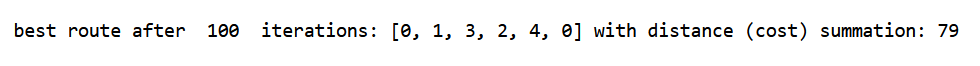
\includegraphics[scale=0.55]{2947_thesis/pictures/ex7.png} 
    \caption{Εκτέλεση με επιστροφή μυρμηγκιού στην αρχική του κορυφή.}
    \label{exret}
\end{figure}

Γίνεται εύκολα κατανοητό ότι το πρόβλημα του πλανόδιου πωλητή, που ξεκινάει από την πόλη όπου βρίσκεται με στόχο να περάσει όλες τις πόλεις με πελάτη και να γυρίσει στην αρχική το συντομότερο δυνατό επισκεπτόμενος κάθε πόλη με πελάτη μόνο μία φορά, ο αλγόριθμος της αποικίας των μυρμηγκιών μπορεί να το προσομοιώσει ικανοποιητικά. 
Αυτό γίνεται αν υποθέσουμε ότι ο γράφος $G=(V(G), E(G))$  που είδαμε παραπάνω αντιπροσωπεύει ένα χάρτη με πόλεις ($V(G)$) και δρόμους ($E(G)$) (σημείωση ότι εάν το γράφημα δεν είναι πλήρες, δηλαδή δεν υπάρχουν δρόμοι που να ενώνουν όλες τις πόλεις, προσθέτουμε ακμές έτσι ώστε να γίνει με βάρος αρκετά μεγάλο καθιστώντας το απίθανο να επιλεγεί ως βέλτιστη λύση, όπως προτείνεται από \lt{Dorigo} και \lt{Stützle} στο \cite{dorigo2004ant}). Σε κάθε δρόμο ($E(G)$) ανατίθεται και ένα κόστος που αντιπροσωπεύει την απόσταση μεταξύ δύο πόλεων, αυτό μπορούμε να το προσαρμόσουμε ανάλογα με την επιθυμία του πωλητή να ακολουθήσει μία διαδρομή (αν για παράδειγμα ο δρόμος είναι ανηφορικός και είναι με τα πόδια), την κίνηση σε κάθε δρόμο (αν είναι με όχημα) και από πολλούς άλλους παράγοντες. Για λόγους απλότητας θα χρησιμοποιηθεί μόνο η απόσταση. Ο στόχος στο πρόβλημα του πλανόδιου πωλητή είναι η εύρεση του ελάχιστου σε απόσταση κύκλου Hamilton στο γράφο-χάρτη. Ενας κύ- κλος Hamilton είναι ένα μονοπάτι που επισκέπτεται κάθε πόλη μία φορά και καταλήγει στην αρχική \cite{dorigo2004ant}.

Για την εκτέλεση του αλγορίθμου που υλοποιήθηκε παραπάνω με στόχο την επίλυση του προβλήματος του πλανόδιου πωλητή πρέπει ο πίνακας με το κόστος κάθε διαδρομής (\lt{distance}) να αντιπροσωπεύει πόλεις και τις αντίστοιχες αποστάσεις μεταξύ τους. Ας πάρουμε για παράδειγμα τον χάρτη\footnote{εικόνα από \lt{google maps} με προσθήκη σημείων} στο σχήμα \ref{map2}, έχουμε 5 πόλεις (areas) που θέλουμε να επισκεφτεί ο πλανόδιος πωλητής, οι οποίες είναι:
\begin{enumerate}
    \item Τρίκαλα
    \item Λάρισα
    \item Κοζάνη
    \item Ιωάννινα
    \item Γρεβενά
\end{enumerate}
\begin{figure}
    \centering
    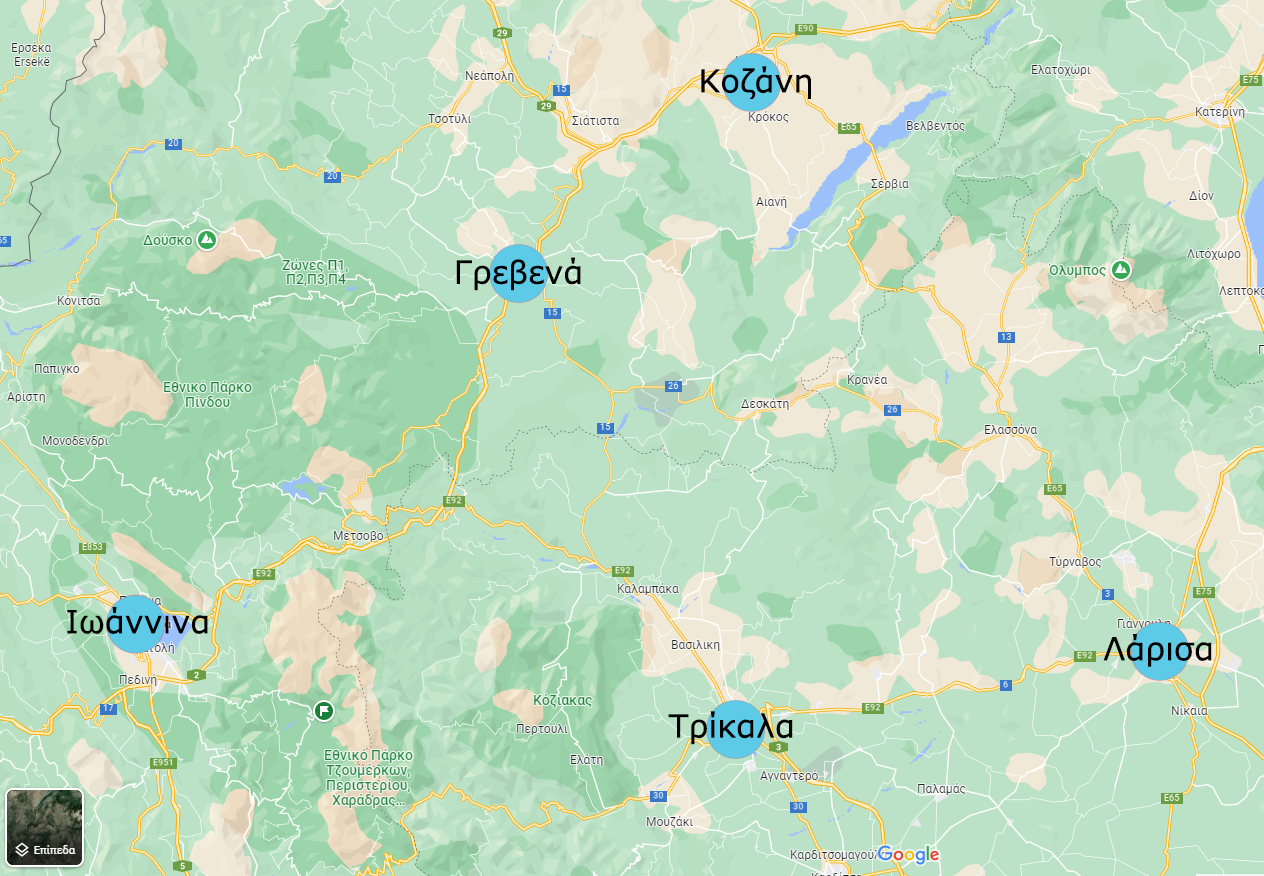
\includegraphics[scale=0.45]{2947_thesis/pictures/map2.png} 
    \caption{Χάρτης με 5 πόλεις που μας ενδιαφέρουν (\lt{cities}).}
    \label{map2}
\end{figure}
Ο χάρτης αυτός μεταφράζεται σε \lt{python} με χρήση της βιβλιοθήκης "\lt{matplotlib}" όπως φαίνεται στο σχήμα \ref{map1}.
\lstinputlisting[language=python]{code/map.py}

\begin{figure}
    \centering
    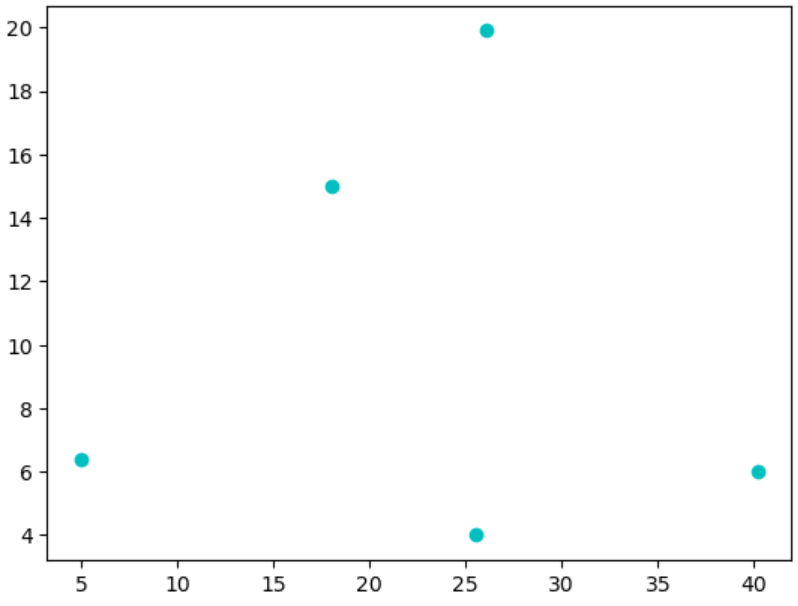
\includegraphics[scale=0.45]{2947_thesis/pictures/map1.png} 
    \caption{Οπτικοποίηση των 5 πόλεων.}
    \label{map1}
\end{figure}

Για να υπολογίσουμε την απόσταση αυτών των πόλεων (\lt{distance}), χωρίς να λαμβάνουμε υπόψιν μας τους δρόμους, θα χρησιμοποιήσουμε τον τύπο της απόστασης μεταξύ δύο σημείων $A(x_1,y_1)$ και $B(x_2,y_2)$, ο οποίος είναι: 
\begin{center}
   $distance(AB) = \sqrt{(x_2-x_1)^2+(y_2-y_1)^2}$ 
\end{center}
Με χρήση αυτού θα υπολογίσουμε την απόσταση κάθε πόλης μεταξύ των υπολοίπων (\lt{distance}), σε κώδικα αυτό υλοποιείται ως εξής:
\lstinputlisting[language=python]{code/dist_cord.py}

Εκτελώντας τον αλγόριθμό μας με τον νέο πίνακα \lt{distance} που εκφράζει τις πόλεις που αναφέραμε, έχουμε ως καλύτερη διαδρομή την $[0, 1, 2, 4, 3, 0]$ όπως φαίνεται και στα σχήματα \ref{best_route}, \ref{best_route_explained}. Οπτικοποίηση των αποτελεσμάτων με χρήση του κώδικα παρακάτω\footnote{εμπνευσμένος από: \url{https://gist.github.com/payoung/6087046}.}, φαίνονται στα σχήματα \ref{route} και \ref{route2}.

\begin{figure}
    \centering
    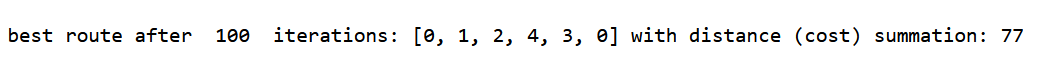
\includegraphics[scale=0.58]{2947_thesis/pictures/best_route.png} 
    \caption{Η καλύτερη διαδρομή.}
    \label{best_route}
\end{figure}
\begin{figure}
    \centering
    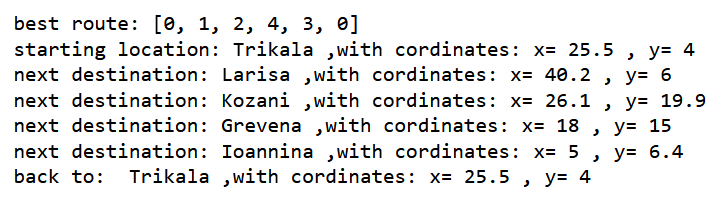
\includegraphics[scale=0.80]{2947_thesis/pictures/best_route_explained.png} 
    \caption{Η καλύτερη διαδρομή αναλυτικά.}
    \label{best_route_explained}
\end{figure}

\lstinputlisting[language=python]{code/visualisation.py}
\begin{figure}
    \centering
    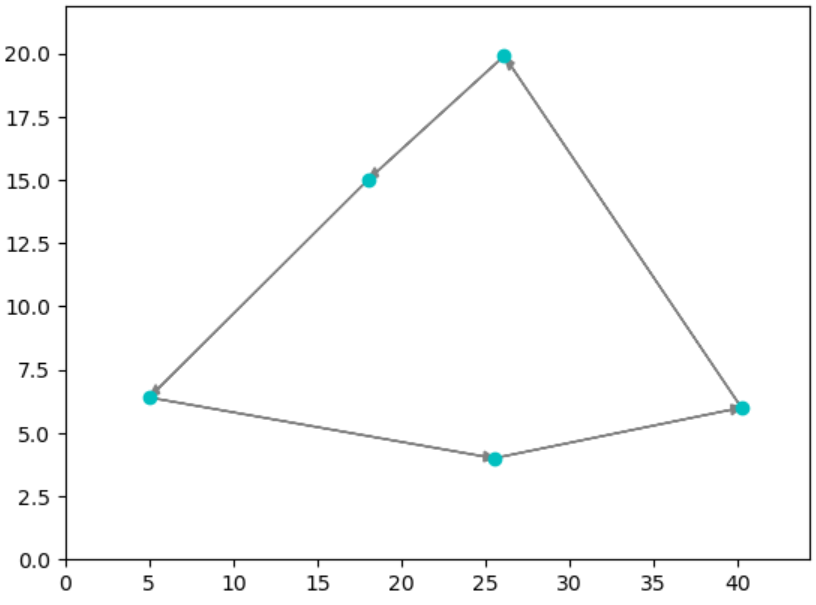
\includegraphics[scale=0.60]{2947_thesis/pictures/route.png} 
    \caption{Η διαδρομή.}
    \label{route}
\end{figure}
\begin{figure}
    \centering
    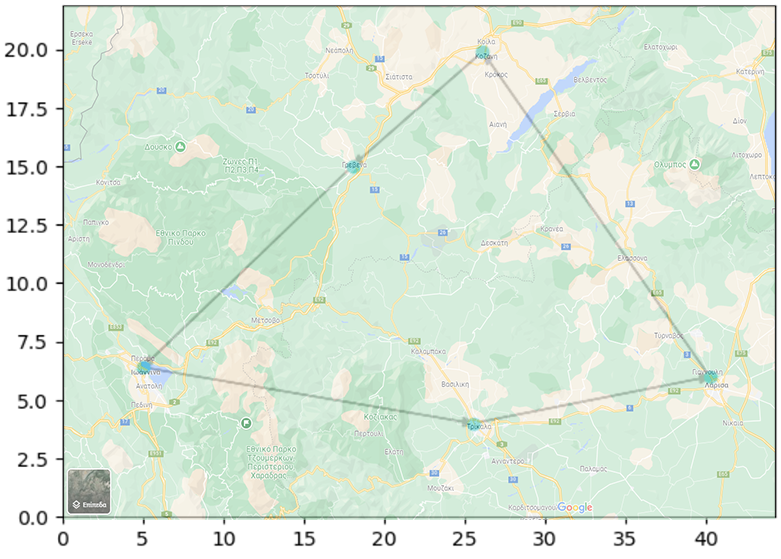
\includegraphics[scale=0.60]{2947_thesis/pictures/route2.png} 
    \caption{Η διαδρομή με τον χάρτη.}
    \label{route2}
\end{figure}

Παρατηρώντας τ' αποτελέσματα, βλέπουμε ότι ο αλγόριθμος δουλεύει όπως θα έπρεπε και μας εξάγει τα βέλτιστα. Μοντελοποίηση του προβλήματος αυτού μπορεί να γίνει με πολλούς άλλους τρόπους ανάλογα από τις απαιτήσεις μας. Στο δικό μας παράδειγμα, η εύρεση της βέλτιστης διαδρομής γίνεται με μοναδικό κριτήριο επιρροής την απόσταση δύο σημείων, χωρίς καν να λαμβάνονται υπόψιν οι δρόμοι. Αυτό μπορεί να γίνει με χρήση γεωχωρικών δεδομένων, όπως για παράδειγμα ενός '\lt{GeoJson}' αρχείου\footnote{\lt{GeoJson} με τον χάρτη της Ελλάδος: \url{https://github.com/codeforgermany/click_that_hood/blob/main/public/data/greece-prefectures.geojson}.}.

\subsubsection{Δρομολόγηση σε δίκτυα δεδομένων}
Ένα ακόμα πρόβλημα που μπορούμε να εφαρμόσουμε τον αλγόριθμο αποικίας μυρμηγκιών είναι αυτό της δρομολόγησης σε δίκτυα δεδομένων (routing in data networks) \cite{bertsekas1998network, dorigo2003ant, di1998antnet}, όπως για παράδειγμα το \lt{AntNet}, που παρουσιάστηκε από τους \lt{Gianni Di Caro} και \lt{Marco Dorigo} στο \cite{di1998antnet}. Η προσέγγιση αυτή, εμπνευσμένη από τον αλγόριθμο που μελετάμε, είναι μια μέθοδος προσαρμοστικής "μάθησης" πινάκων δρομολόγησης σε δίκτυα δεδομένων.

Ο στόχος ενός αλγορίθμου δρομολόγησης σε δίκτυα δεδομένων είναι να κατευθύνει τη ροή των δεδομένων από την κορυφή προέλευσης στην κορυφή προορισμού μεγιστοποιώντας την απόδοση \cite{di1998antnet}. Έστω ο κατευθυνόμενος γράφος $G(V,E)$, όπου $G$ αντιπροσωπεύει ένα δίκτυο με κορυφές-$V$ να εκφράζουν την μονάδα επεξεργασίας ή προώθησης και ακμές-$E$ το σύστημα μετάδοσης. Σε κάθε κορυφή $V$, ουσιαστικά, λαμβάνεται μια απόφαση σχετικά με την προώθηση του κάθε πακέτου δεδομένων στον προορισμό του. Αυτή η απόφαση εξαρτάται από πληροφορίες σχετικά με την κατάσταση (κίνηση-\lt{traffic}) του δικτύου που δημιουργείται από τους χρήστες (\lt{user-generated traffic}) \cite{di1998antnet}. Η φερομόνη (\lt{pheromone}) που παράγεται εκφράζει πληροφορίες όπως η ποιότητα της διαδρομής που βρέθηκε σε αυτό το δίκτυο, η καθυστέρηση στην μετάδοση των δεδομένων, και άλλα. Τα μυρμήγκια (\lt{ants}), σε αυτό το πρόβλημα, βρίσκουν σταδιακά λύσεις χρησιμοποιώντας αυτές τις πληροφορίες. Αυτό έχει ως αποτέλεσμα το δίκτυο να προσαρμόζεται στις μεταβαλλόμενες συνθήκες και να βρίσκει τις βέλτιστες διαδρομές για την μετάδοση των δεδομένων μεταξύ δύο κορυφών \cite{dorigo2003ant}. 


\subsubsection{Επεξεργασία εικόνας}
Ένας ακόμα κλάδος που μπορεί να γίνει εφαρμογή του αλγόριθμου της αποικίας των μυρμη- γκιών είναι αυτός της επεξεργασίας εικόνας. Αν και ο αλγόριθμος αυτός δεν είναι κατ' αυτού σχεδιασμένος για την επεξεργασία εικόνας, μπορεί να χρησιμοποιηθεί για ορισμένες εφαρμογές. Πιο συγκεκριμένα, μπορεί να επιτευχθεί ανίχνευση ακμών και αντικειμένων ή και να βελτιωθεί η ποιότητα της ως προς το χρώμα, την φωτεινότητα και την αντίθεση, δείτε \cite{mpikou2013euretikoi, nezamabadi2006edge, baterina2010image, tian2008ant}. Αυτή η διαδικασία έχει ως στόχο την εύρεση των ορίων ενός αντικειμένου σε μία εικόνα και μπορεί να χρησιμοποιηθεί σε εφαρμογές μηχανικής όρασης (\lt{machine vision}) και ανάλυσης εικόνας \cite{baterina2010image}. 

Μια προσέγγιση με τον αλγόριθμο της αποικίας των μυρμηγκιών για την επίτευξη αυτού, μπορεί να γίνει θεωρώντας την εικόνα μας ως ένα γράφο, με τα φωτεινότητα των \lt{pixels} της σε κάθε ακμή (\lt{edge}) του γράφου. Οι ακμές ενώνουν γειτονικά \lt{pixels}, δηλαδή ο γράφος μας δεν είναι πλήρως συνδεδεμένος. Το κάθε μυρμήγκι προχωράει από \lt{pixel} σε \lt{pixel} επηρεασμένο από την τιμή φωτεινότητας που υπάρχει στις ακμές (edges) του γράφου. Στόχος των μυρμηγκιών είναι η δημιουργία ενός πίνακα με φερομόνες που θα αντιστοιχεί με τις ακμές/αντικείμενα της εικόνας μας \cite{baterina2010image, nezamabadi2006edge, tian2008ant}. 


